
%%%%%%%%%%%%%%%%%%%%%%%%%%%%% Define Article %%%%%%%%%%%%%%%%%%%%%%%%%%%%%%%%%%
\documentclass[conference]{IEEEtran}
%%%%%%%%%%%%%%%%%%%%%%%%%%%%%%%%%%%%%%%%%%%%%%%%%%%%%%%%%%%%%%%%%%%%%%%%%%%%%%%

%%%%%%%%%%%%%%%%%%%%%%%%%%%%% Using Packages %%%%%%%%%%%%%%%%%%%%%%%%%%%%%%%%%%
\usepackage{geometry}
\usepackage{graphicx}
\usepackage{amssymb}
\usepackage{amsmath}
\usepackage{amsthm}
\usepackage{empheq}
\usepackage{mdframed}
\usepackage{booktabs}
\usepackage{lipsum}
\usepackage{graphicx}
\usepackage{color}
\usepackage{psfrag}
\usepackage{pgfplots}
\usepackage{bm}
\usepackage[spanish]{babel}
\usepackage[utf8]{inputenc} % Codificación UTF,8
\usepackage{amsmath}        % Soporte para ecuaciones matemáticas
\usepackage{graphicx}       % Manejo de imágenes
\usepackage{hyperref}       % Hipervínculos
\usepackage{caption}        % Formato para figuras
\usepackage{multirow}
\usepackage{subcaption}
\usepackage{biblatex}
\addbibresource{ref/cable.bib} % Add the bibliography file in the preamble (correct usage)
\usepackage{csquotes}
\usepackage{bookmark}
%%%%%%%%%%%%%%%%%%%%%%%%%%%%%%%%%%%%%%%%%%%%%%%%%%%%%%%%%%%%%%%%%%%%%%%%%%%%%%%

% Other Settings

%%%%%%%%%%%%%%%%%%%%%%%%%% Page Setting %%%%%%%%%%%%%%%%%%%%%%%%%%%%%%%%%%%%%%%
\geometry{a4paper, margin=1in}

%%%%%%%%%%%%%%%%%%%%%%%%%% Define some useful colors %%%%%%%%%%%%%%%%%%%%%%%%%%
\definecolor{ocre}{RGB}{243,102,25}
\definecolor{mygray}{RGB}{243,243,244}
\definecolor{deepGreen}{RGB}{26,111,0}
\definecolor{shallowGreen}{RGB}{235,255,255}
\definecolor{deepBlue}{RGB}{61,124,222}
\definecolor{shallowBlue}{RGB}{235,249,255}
%%%%%%%%%%%%%%%%%%%%%%%%%%%%%%%%%%%%%%%%%%%%%%%%%%%%%%%%%%%%%%%%%%%%%%%%%%%%%%%

%%%%%%%%%%%%%%%%%%%%%%%%%% Define an orangebox command %%%%%%%%%%%%%%%%%%%%%%%%
\newcommand\orangebox[1]{\fcolorbox{ocre}{mygray}{\hspace{1em}#1\hspace{1em}}}
%%%%%%%%%%%%%%%%%%%%%%%%%%%%%%%%%%%%%%%%%%%%%%%%%%%%%%%%%%%%%%%%%%%%%%%%%%%%%%%

%%%%%%%%%%%%%%%%%%%%%%%%%%%% English Environments %%%%%%%%%%%%%%%%%%%%%%%%%%%%%
\newtheoremstyle{mytheoremstyle}{3pt}{3pt}{\normalfont}{0cm}{\rmfamily\bfseries}{}{1em}{{\color{black}\thmname{#1}~\thmnumber{#2}}\thmnote{\,,,\,#3}}
\newtheoremstyle{myproblemstyle}{3pt}{3pt}{\normalfont}{0cm}{\rmfamily\bfseries}{}{1em}{{\color{black}\thmname{#1}~\thmnumber{#2}}\thmnote{\,,,\,#3}}
\theoremstyle{mytheoremstyle}
\newmdtheoremenv[linewidth=1pt,backgroundcolor=shallowGreen,linecolor=deepGreen,leftmargin=0pt,innerleftmargin=20pt,innerrightmargin=20pt,]{theorem}{Theorem}[section]
\theoremstyle{mytheoremstyle}
\newmdtheoremenv[linewidth=1pt,backgroundcolor=shallowBlue,linecolor=deepBlue,leftmargin=0pt,innerleftmargin=20pt,innerrightmargin=20pt,]{definition}{Definition}[section]
\theoremstyle{myproblemstyle}
\newmdtheoremenv[linecolor=black,leftmargin=0pt,innerleftmargin=10pt,innerrightmargin=10pt,]{problem}{Problem}[section]
%%%%%%%%%%%%%%%%%%%%%%%%%%%%%%%%%%%%%%%%%%%%%%%%%%%%%%%%%%%%%%%%%%%%%%%%%%%%%%%

%%%%%%%%%%%%%%%%%%%%%%%%%%%%%%% Plotting Settings %%%%%%%%%%%%%%%%%%%%%%%%%%%%%
\usepgfplotslibrary{colorbrewer}
\pgfplotsset{width=8cm,compat=1.9}
%%%%%%%%%%%%%%%%%%%%%%%%%%%%%%%%%%%%%%%%%%%%%%%%%%%%%%%%%%%%%%%%%%%%%%%%%%%%%%%

%%%%%%%%%%%%%%%%%%%%%%%%%%%%%%% Title & Author %%%%%%%%%%%%%%%%%%%%%%%%%%%%%%%%
\author{\IEEEauthorblockN{Daniel Fernando Aranda Contreras, Carlos Fernando Torres Ferrer}
\IEEEauthorblockA{Escuela E3T, Universidad Industrial de Santander\\
Correo electrónico: \{daniel2221648, carlos2221116 \}@correo.uis.edu.co}}

%%%%%%%%%%%%%%%%%%%%%%%%%%%%%%%%%%%%%%%%%%%%%%%%%%%%%%%%%%%%%%%%%%%%%%%%%%%%%%%
    \begin{document}
        % Título
        \title{\uppercase{Diseño y construcción de un transformador eléctrico}}
        \maketitle
        % Resumen
        % Palabras clave        
        \begin{IEEEkeywords}
            Transformador
            Tensión,
            Bobinado,
            Relación de transformación,
            Aislante,
            Fusibles,
            Corriente,
            Potencia,
            Diseño,
            Construcción.
        \end{IEEEkeywords}



        \begin{abstract}
            For this activity, "Design and Construction of an Electrical Transformer," in the subject Electrical Machines I, which aims to improve ABET student outcome 6: "Ability to develop and conduct appropriate experiments, analyze and interpret data, and use engineering judgment to draw conclusions." The objective is to construct a transformer model that will be evaluated against rubric. Therefore, the following report will detail the transformer design, including its dimensions, coil gauge, number of turns in each winding, etc. The details and results of voltage, current, and power obtained through short-circuit and open-circuit tests in the High Voltage laboratories will also be specified.
        \end{abstract}
        %\section{Objetivos} 
\begin{itemize}
    \item Realizar las pruebas de vacío y de cortocircuito en un transformador monofásico configurado como autotransformador para analizar su comportamiento eléctrico.
    \item Determinar experimentalmente el rendimiento y la regulación del autotransformador bajo diferentes tipos de carga: resistiva, inductiva y capacitiva.
\end{itemize}

\section{Equiops y materiales}
\begin{itemize}
    \item Transformador monofásico.
    \item Voltímetro CA.
    \item Amperímetro CA.
    \item Vatímetro monofásico CA.
    \item Transformador de corriente (CT).
    \item Cargas: resistivas (R), inductivas (L) y capacitivas (C).
\end{itemize}

\section{Introducción}
\text{Los autotransformadores son dispositivos eléctricos que facilitan la modificación de los niveles de tensión dentro de un rango específico de manera eficiente. A diferencia de los transformadores tradicionales, en los autotransformadores los devanados primario y secundario no están completamente aislados, ya que comparten una parte del mismo arrollamiento. Esto resulta en una reducción del material conductor utilizado y en una mejora de la eficiencia del sistema. En este laboratorio, se realizará un estudio de un transformador monofásico funcionando como autotransformador, a través de pruebas experimentales que permitirán evaluar su rendimiento y regulación en diversas condiciones de carga.}

\section{Conclusión}
\text{A lo largo del laboratorio, se estudió el comportamiento de un transformador monofásico operando como autotransformador, evaluando su rendimiento y regulación bajo diferentes condiciones de carga, las cuales tienen una gran influencia en su rendimiento depediendo el tipo de carga, si es una carga RC conectada en paralelo tiende a aunmentar su tension de salida en comparacion con una carga netamente resistiva, mientras que con una carga inductiva conectada en serie su nivel de tension de salida disminuye, pero si conectamos una carga RLC está tiene un comportamiento de compensacion, si las cargas inductivas (L) y capacitivas (C) tienen valores similares.}
        \section{Introducción}
Los transformadores se han convertido en parte esencial de nuestro día a día, los podemos encontrar en muchos lados, incluso en nuestras casas, estos dispositivos permiten hacer el cambio de tensión para facilitar el manejo de esta, podemos encontrarlo en cargadores cuya función es reducir la tensión para el correcto funcionamiento y evitando el daño del dispositivo a cargar, se encuentran también en las ciudades donde su función es disminuir la tensión para el uso comercial o para el uso doméstico, así como el transformador puede ser un reductor también puede ser elevador, este transformador es principalmente utilizado en el principio de la cadena de producción de energía eléctrica, su función es elevar la tensión a cierto punto en el cual permite la transmisión de energía disminuyendo en gran medida sus pérdidas.

\section{Resumen}
Para esta actividad “Diseño y construcción de un transformador eléctrico” de la asignatura máquinas eléctricas I que tiene como finalidad mejorar el student outcome 6 del ABET: “Capacidad para desarrollar y llevar una experimentación adecuada, analizar e interpretar datos y usar juicios de ingeniería para sacar conclusiones.”, se requiere como finalidad construir un modelo de transformador que será evaluado con respecto a una rúbrica, por lo cual, en el siguiente informe se detalla a fondo el diseño del transformador, como lo son sus dimensiones, el calibre de sus bobinas, el número de vueltas de cada bobinado, etc. Así como también se va a especificar los detalles y resultados de tensión, corriente y potencia, los cuales fueron obtenidos por medio de las pruebas de corto circuito y de circuito abierto en los laboratorios de Alta Tensión.

        \section{Principio de funcionamiento} 
Si bien en el diseño no se tiene un transformador ideal, es importante entender el principio de funcionamiento de un transformador ideal, ya que este nos permite acercarnos a el funcionamiento del transformador real y de allí pasar al diseño del tramsformador.

\subsection{Transformador ideal}

\begin{figure}[ht!]
    \centering
    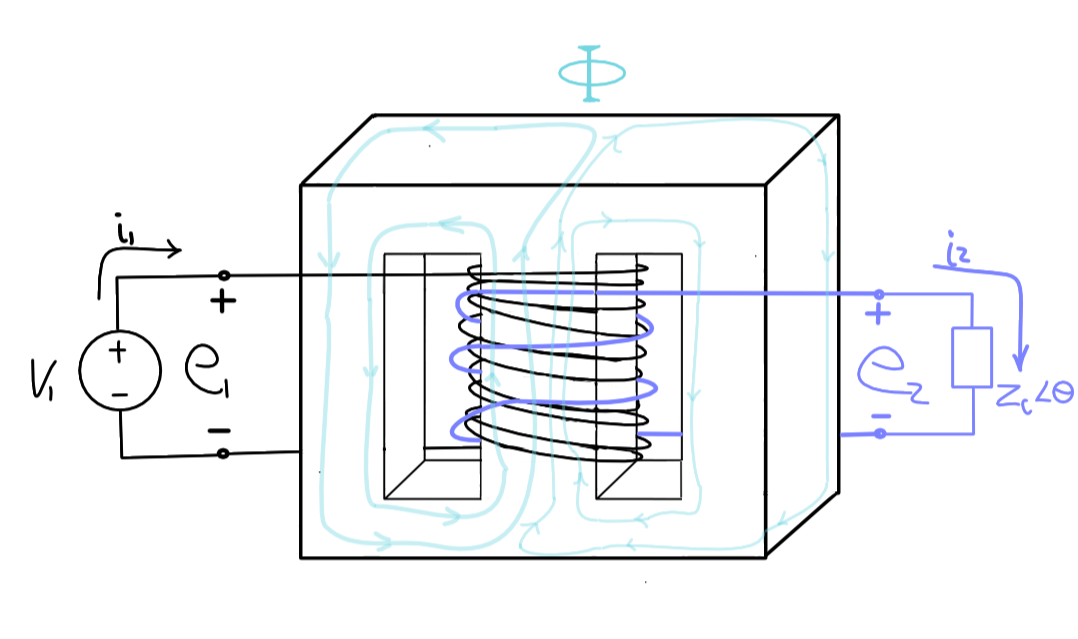
\includegraphics[width=0.48\textwidth]{fot/T4.png}
    \caption{Modelo de tramsformador ideal.}
    \label{fig:T4}
\end{figure}

A partir de la ley de Faraday-Lenz, se establece que la fuerza electromotriz (fem) inducida en un circuito es proporcional a la rapidez de cambio del flujo magnético a través de él. Resultado para una bobina La ecuación que describe esta relación es la siguiente:
\begin{equation}
    \label{eqn1}
    e_1 = N_1 \cdot \frac{d\Phi}{dt}
\end{equation}


\addcontentsline{toc}{section}{Nomenclature}
\begin{IEEEdescription}[\IEEEsetlabelwidth{$V_1,V_2,$}]
\item[e] F.e.m inducida en la bobina.
\mbox{}
\item[$N$] Número de vueltas de la bobina.
\item[$\Phi$] Flujo magnético a través de la bobina.
\end{IEEEdescription}

\vspace{0.5cm}
Si se tiene que la fuente es una sinusoide, el flujo magnético es:
\begin{equation}
    \Phi = \Phi_m \cdot \sin(\omega t)
\end{equation}

Puesto que es un transformador ideal, la f.e.m. inducida en el primario es igual a la tensión de entrada, por lo que se puede escribir la ecuación \ref{eqn1} como:

\begin{center}
    $V_1 = N_1 \cdot \frac{d\Phi}{dt} = N_1 \cdot \frac{d}{dt}(\Phi_m \cdot \sin(\omega t))$
    \\
    $= N_1 \cdot \Phi_m \cdot \omega \cdot \cos(\omega t) [V]$
    \\
    $V_1 = \frac{N_1 \cdot \Phi_m \cdot \omega}{\sqrt{2}}\cdot  [Vrms]$
\end{center}
\begin{equation}
    \label{eqn2}
    V_1 =N_1 \cdot \Phi_m \cdot \frac{f \cdot 2\pi}{\sqrt{2}} [Vrms]
\end{equation}
\vspace{0.3cm}

Tenemos la ley de Gauss para campo magnético, que establece que el flujo magnético a través de una superficie cerrada es igual a la integral de la densidad de flujo magnético a través de esa superficie. La ecuación que describe esta relación es la siguiente:
\begin{equation}
    \label{eqn3}
    \Phi = \int_S \mathbf{B} \cdot d\mathbf{S}
\end{equation}
Como la sección transversal del núcleo es cuadrada, se puede escribir la ecuación \ref{eqn3} como: $\Phi = B \cdot S$
\\
Finalmente de la ecuación \ref{eqn3} en \ref{eqn2} despejando para N se obtiene:
\\
\begin{equation}
    \label{eqn4}
    N_1 = \frac{V_{1rms}}{\Phi_m \cdot f \cdot \frac{2\pi}{\sqrt{2}}} = \frac{V_{1rms}}{B\cdot S\cdot f \cdot \frac{2\pi}{\sqrt{2}}} [vueltas] 
\end{equation}
\\
\addcontentsline{toc}{section}{Nomenclature}
\begin{IEEEdescription}[\IEEEsetlabelwidth{$e,N,S$}]
\item[$f$] frecuencia de la fuente.
\mbox{}
\item[$V_{1rms}$] Tensión eficaz en el primario.
\item[$\Phi$] Flujo magnético a través del arrollamiento.
\item[$B$] densidad de flujo magnético.
\item[$S$] Sección transversal del núcleo. 
\end{IEEEdescription}
\vspace{1cm}


\begin{IEEEeqnarraybox*}{rCl}
    \text{Transformador ideal:} & \text{Transformador real:} \\
    \text{Sin pérdidas} & \text{Con pérdidas} \\
    \text{Sin resistencia} & \text{Con resistencia} \\
    \text{Sin reactancia} & \text{Con reactancia} \\
    \text{Sin saturación} & \text{Con saturación} \\
    \text{Sin fuga de flujo} & \text{Con fuga de flujo}
\end{IEEEeqnarraybox*}
        \section{Diseño y aspectos constructivos del transformador}

\subsection{Núcleo}
Las laminas del nucleo son de acero al silicio laminado en frío. El nucleo esta construido con láminas en forma de E y de I, el transformador se construye con 68 láminas de E y con 66 láminas de I, las cuales al ser acomodadas comprenden una sección transversal de $22 \cdot 38 [mm^{2}]$, la cual es la misma sección transversal de nuestro carrete (la del carrete es un poco mayor).
En la figura \ref{fig:T1} se muestra las dimensiones de las laminas E además de la I del nucleo.
\\\textbf{Disposición de las laminas en el nucleo:} como último paso cuando se tienen las vueltas alrededor del carrete, se posicionan las laminas como se muestra en la figura \ref{fig:T2}. 


\begin{figure}[ht!]
    \centering
    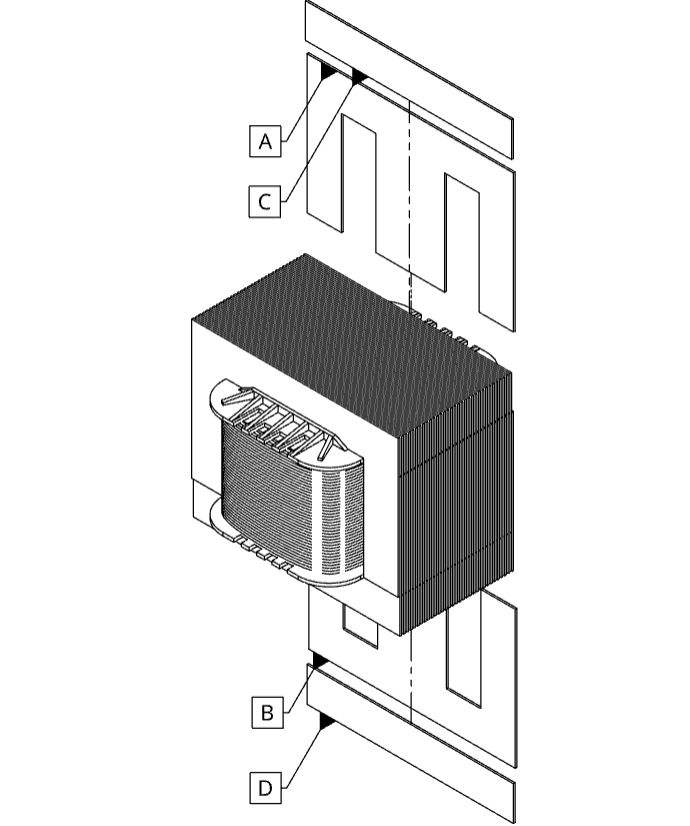
\includegraphics[width=0.48\textwidth]{fot/T2.png}
    \caption{Plano de disposición de las laminas en el nucleo primero se alterna entre el paso A y B sucesivamente hasta que se tenga apretado el carrete y posterior se alterna entre el paso C y D.}
    \label{fig:T2}
\end{figure}



\subsection{Carrete}
El carrete comprende una sección transversal de  $22 \cdot 38 [mm^{2}]$ y una altura de 33 [mm], la sección transversal del carrete es un poco mayor a lo mencionado pero principalmente es igual a la del nucleo, estos datos son necesarios para poder hacer los cálculos del número de vueltas requeridas para el bobinado primario y el bobinado secundario.
En la figura \ref{fig:T1} se muestra las dimensiones de la sección transversal del carrete. 

\begin{figure}[ht!]
    \centering
    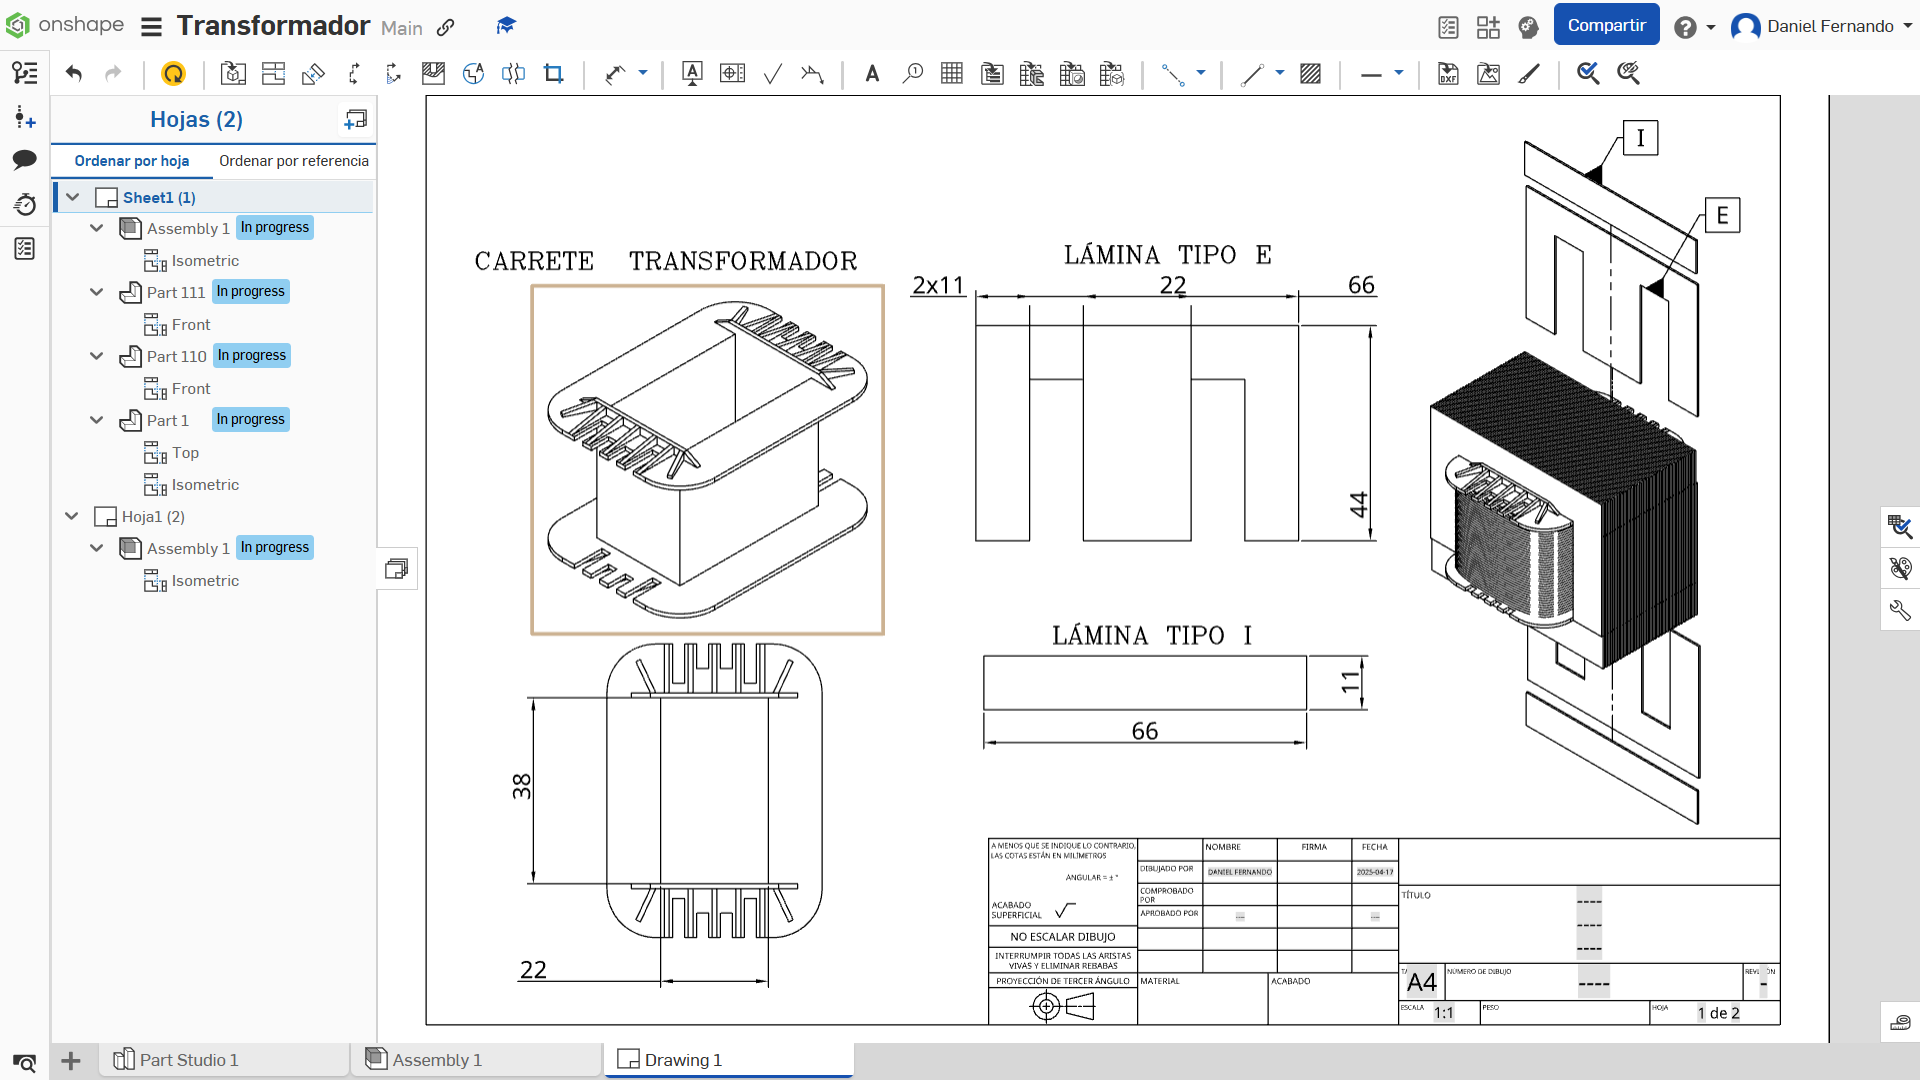
\includegraphics[width=0.48\textwidth]{fot/T1.png}
    \caption{Plano con aspectos constructivos.}
    \label{fig:T1}
\end{figure}



\subsection{Relación de transformación}
Para la relación de transformación elegimos los voltajes de 120 [V] a 50 [V], al realizar la relación de transformación nos queda de la siguiente manera: 

\subsection{Número de vueltas}
Recordando la ecuación \ref{eqn5}
esto nos resultaria en el siguiente numero de vueltas:

\begin{center}
    $N_1 = \frac{\frac{120}{\sqrt{2}}}{1.1\cdot S\cdot f \cdot \frac{2\pi}{\sqrt{2}}\cdot 0.9}=384.599 \approx 385\ [vueltas]$
    $N_2 = \frac{\frac{50}{\sqrt{2}}}{1.1\cdot S\cdot f \cdot \frac{2\pi}{\sqrt{2}}\cdot 0.9}=160.249 \approx 160\ [vueltas]$
    \end{center}
    
\subsection{Bobinado primario}
Teniendo el número de vueltas requerido para el lado primario es de 385, hacemos los cálculos de cuánta corriente podría pasar por el conductor según el voltaje seleccionado 120 [V] y la potencia que queremos 50 [VA], seleccionamos un conductor adecuado el cual es cobre esmaltado de calibre AWG 24 que permite el paso de una corriente de 0.577 A (amperios) a 0.94 A .

\subsection{Bobinado secundario}
Para hallar el número de vueltas que se requiere en el lado secundario lo despejamos de la fórmula de relación de transformación, al aplicarlo tenemos que la cantidad de vueltas será de 160, para este lado secundario también analizamos la corriente que pasará con un voltaje de 50 [V] y una potencia de 50 [VA], seleccionamos un conductor de cobre esmaltado de calibre AWG 22 que permite el paso de una corriente de 0.92 A (amperios) a 1.5 A .

\subsection{Aislante}
Se envolvió entre ambos bobinados una capa de papel aislante, el cual ayuda a cubrir ambos bobinados y separarlos entre ellos.

\subsection{Fusibles}
Se agregaron dos portafusibles, uno en cada borne de alimentación del transformador, es decir, un fusible de 2 [A] en el lado de tensión primario y uno de 5 [A] en el lado de tensión secundario, esto para prevenir posibles quemaduras o fallas en el dispositivo. Y finalmente se realizo toda la conexión con las borneras.



\begin{figure}[ht!]
    \centering
    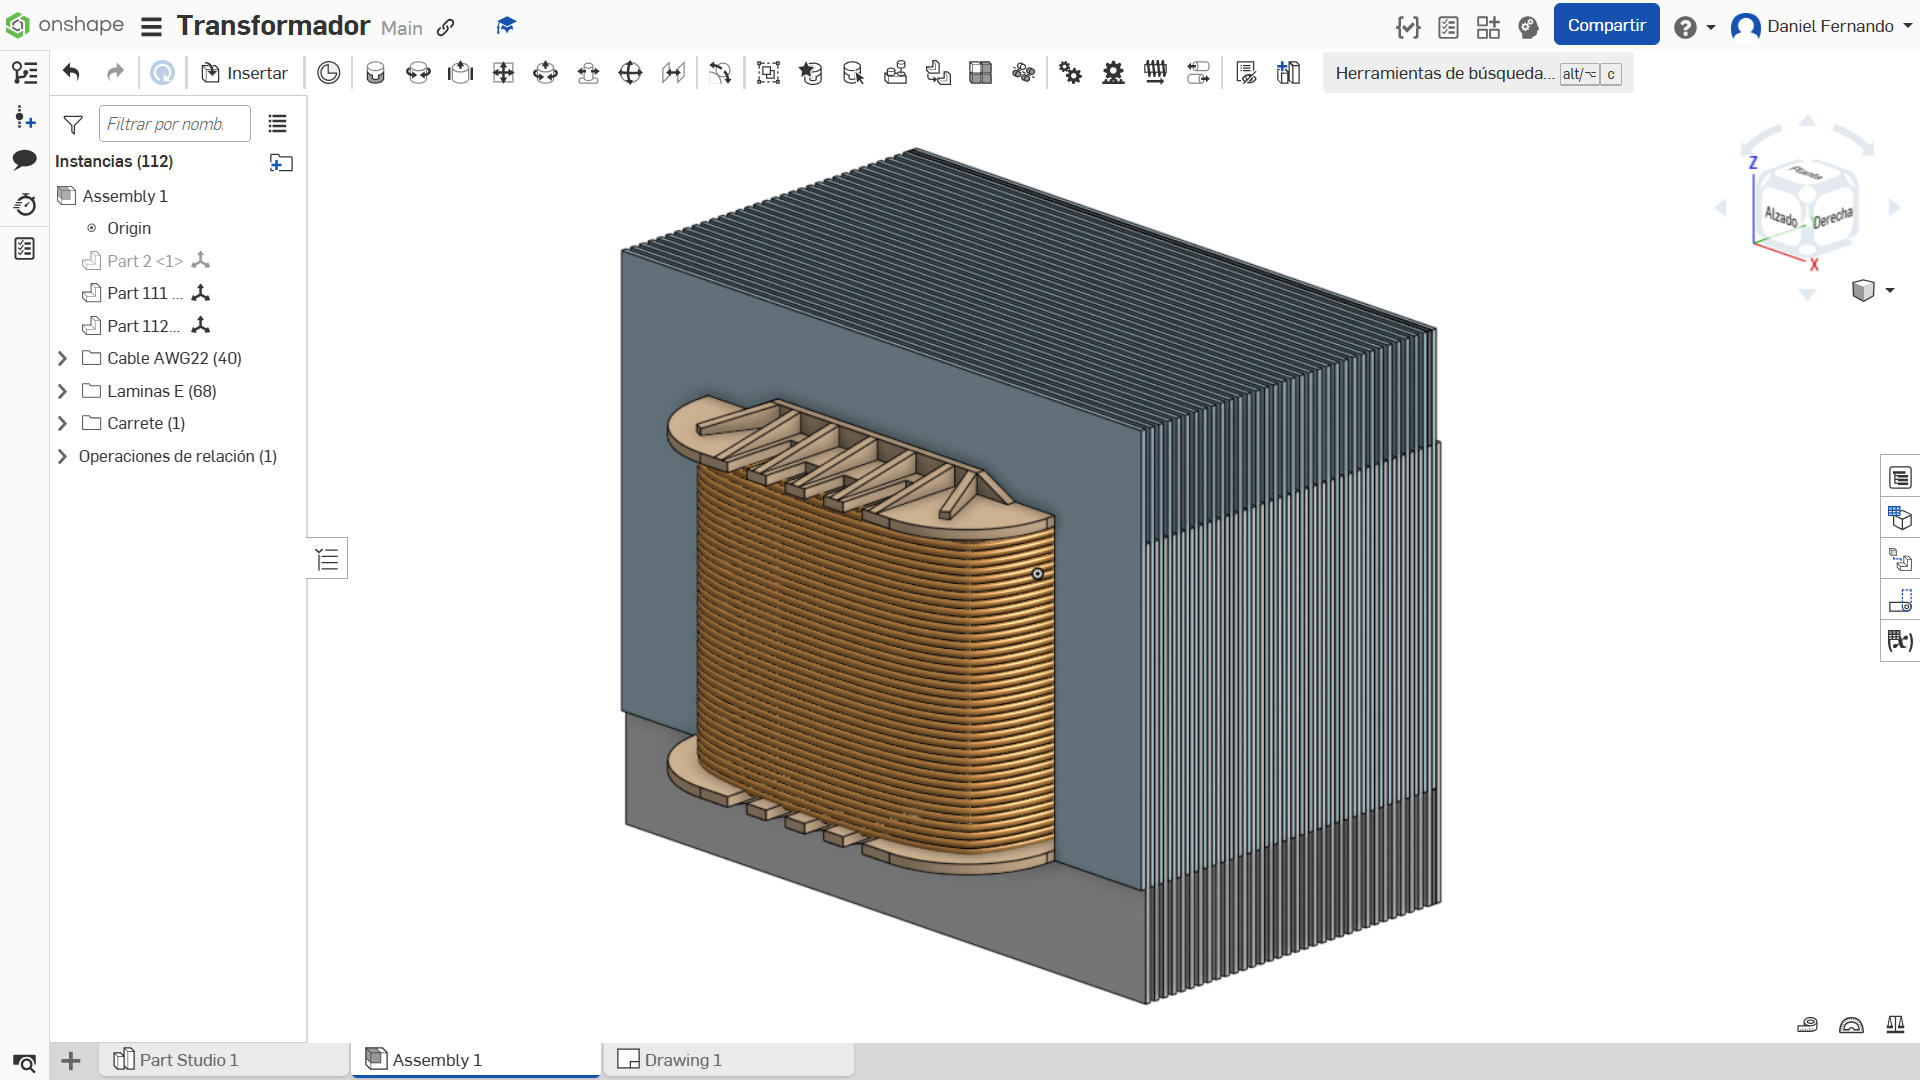
\includegraphics[width=0.48\textwidth]{fot/T3.png}
    \caption{Resultado final del transformador (ocultando los fusibles y el papel aislante).}
    \label{fig:T3}
\end{figure}

|       
\section*{Pruebas de Laboratorio Alta Tensión}

Para probar el funcionamiento de un transformador, es necesario someterlo a un par de pruebas, las cuales son la Prueba de Corto Circuito y la Prueba de Circuito Abierto. Con base en estas dos pruebas podemos ver la relación de tensión entre ambos bobinados, las corrientes que manejan estos y su potencia.

\subsection*{Prueba de Corto Circuito}

Para esta prueba, se cortocircuita uno de los lados del transformador. Se calcula qué corriente pasa por este cortocircuito y qué tensión es la aplicada en el lado primario. Al escoger una potencia de 50 W y tener el lado secundario con una tensión de 50 V, se aplica una corriente por el cortocircuito de 1 A. Por la fórmula (sabiendo que la potencia reactiva de la rama de magnetización es muy ínfima):
\begin{figure}[ht!]
    \centering
    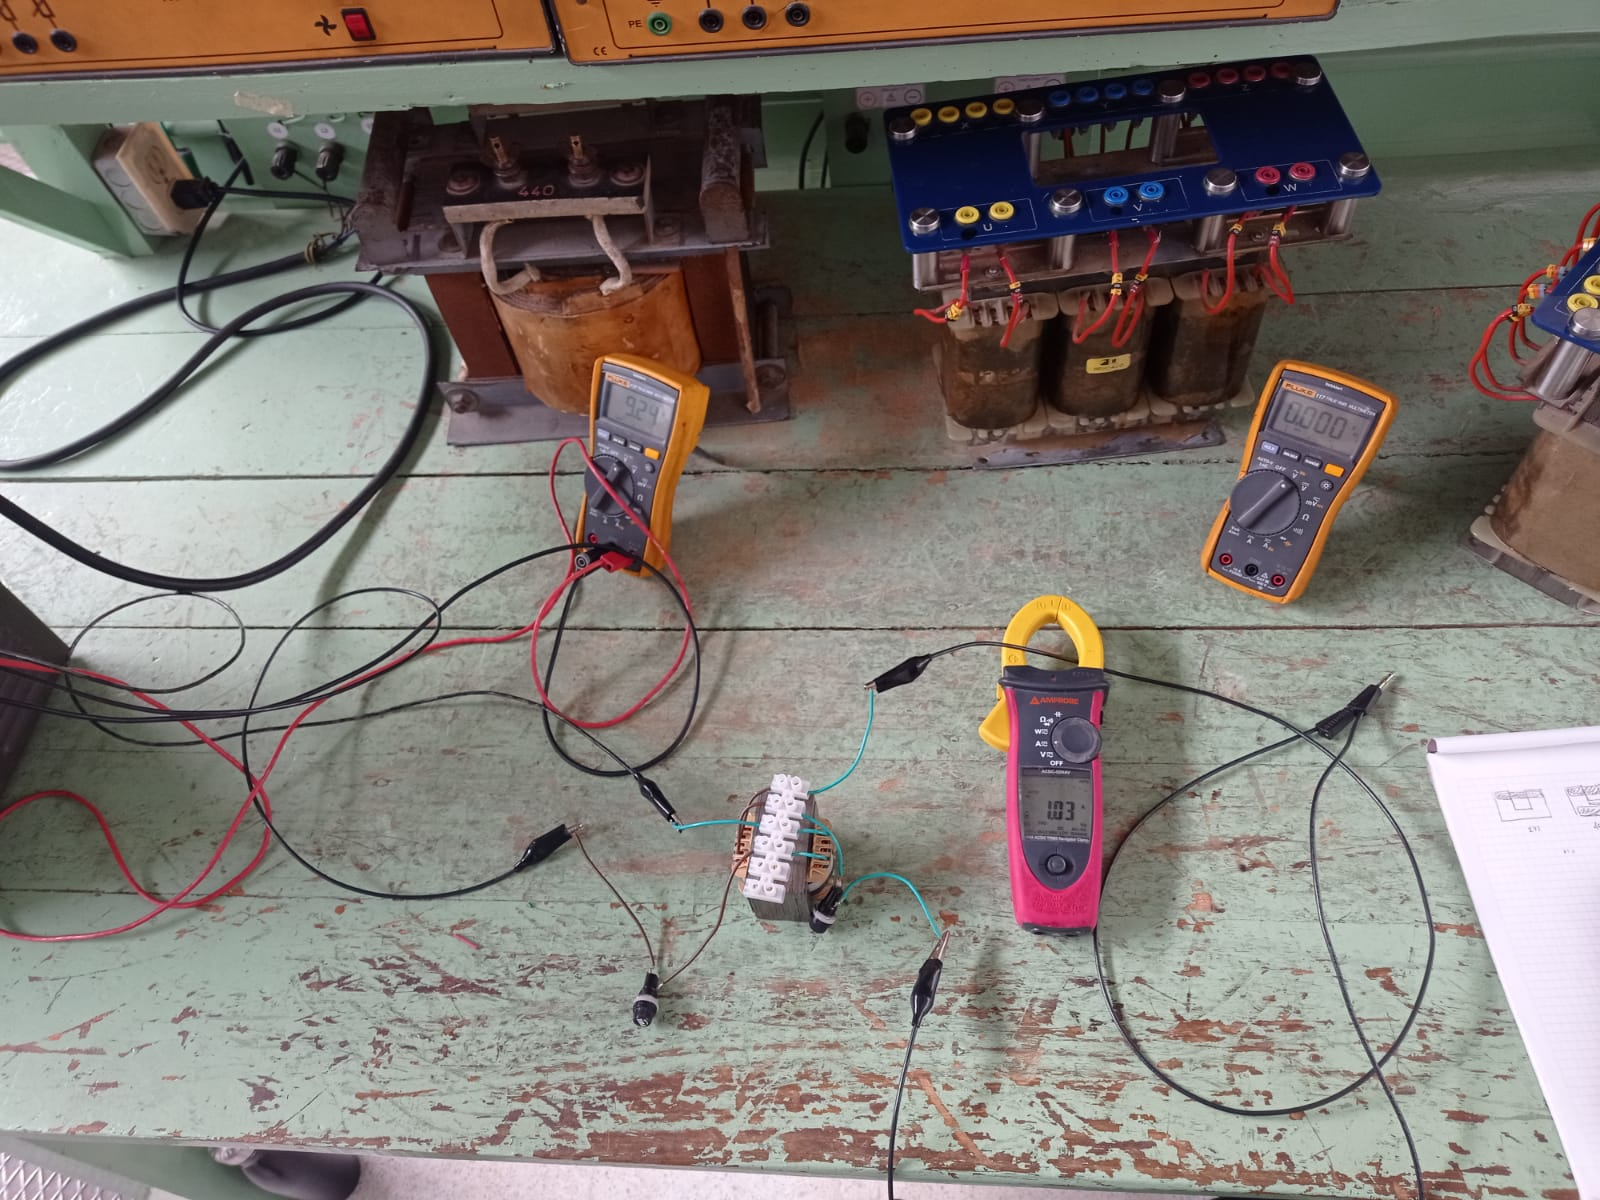
\includegraphics[width=0.48\textwidth]{fot/TP1.jpeg}
    \caption{Prueba en el laboratorio de alta tensión.}
    \label{fig:TP1}
\end{figure}

\begin{center}
    $S = V \cdot I = 50\ [VA]$
\end{center}
Tensión del lado primario:
\begin{center}
    $9.24 [V]$
\end{center}

\begin{center}
    $Corriente \ que \ recorre \ el \ cortocircuito: \ 1.03\ [A]$
\end{center}

\subsection*{Prueba de Circuito Abierto}

En esta prueba, se deja el lado secundario abierto. Se calcula la tensión en este lado y se toman la corriente y la tensión que aplicamos en el lado primario del transformador. Para esta parte del laboratorio se comprueba la relación de transformación, teniendo en cuenta los criterios que escogimos para nuestro transformador, el cual es: tensión del lado primario 120 V y lado secundario 50 V. Aplicamos la fórmula:

Relación de transformación:
\begin{center}
    $\frac{V_p}{V_s} = \frac{120\ [V]}{50\ [V]} = 2.4$
\end{center}


\begin{figure}[ht!]
    \centering
    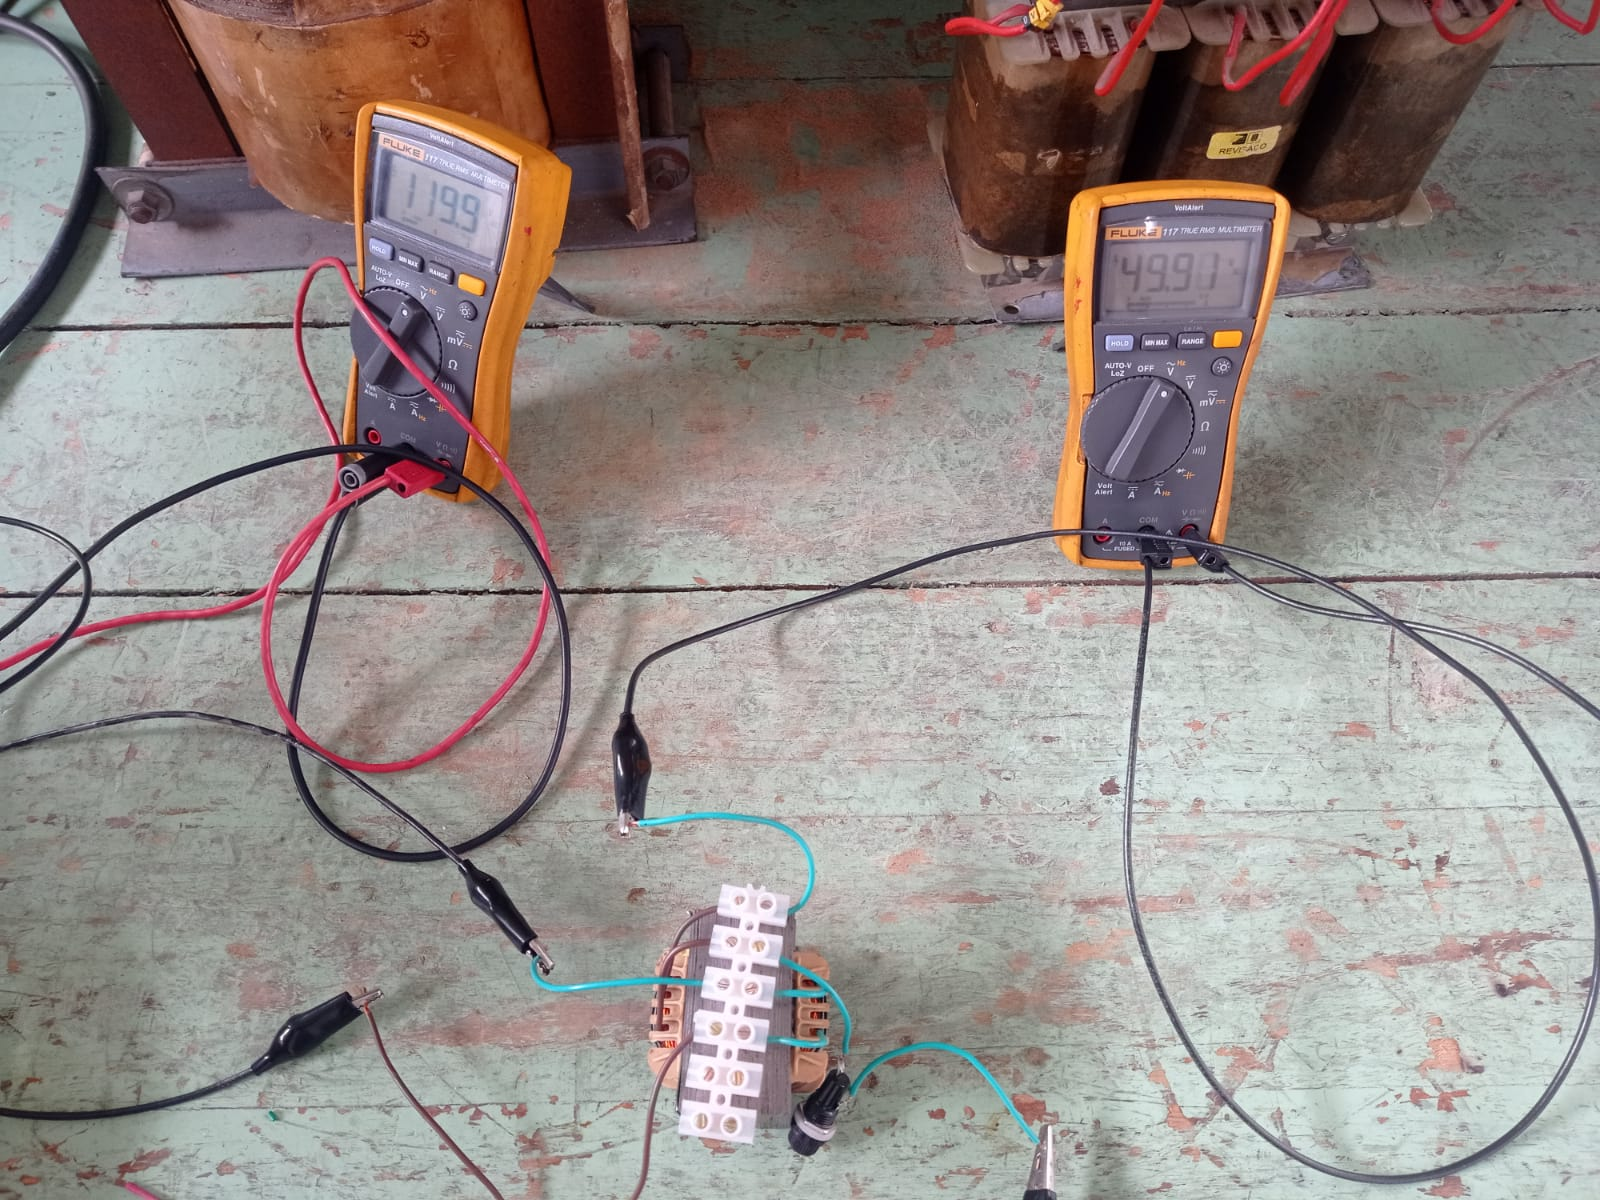
\includegraphics[width=0.48\textwidth]{fot/TP3.jpeg}
    \caption{Prueba en el laboratorio de alta tensión.}
    \label{fig:TP3}
\end{figure}
 
Tensión en el lado primario del transformador:
\begin{center}
    $119.9\ [V]$
\end{center}
Tensión en el lado secundario del transformador: 
\begin{center}
    $49.91\ [V]$
\end{center}
Relación de transformación: 
\begin{center}
    $ \frac{119.9\ [V]}{49.91\ [V]} = 2.402$
\end{center}
Corriente por el lado primario del transformador: 
\begin{center}
    $0.22\ [A]$
\end{center}
\begin{figure}[ht!]
    \centering
    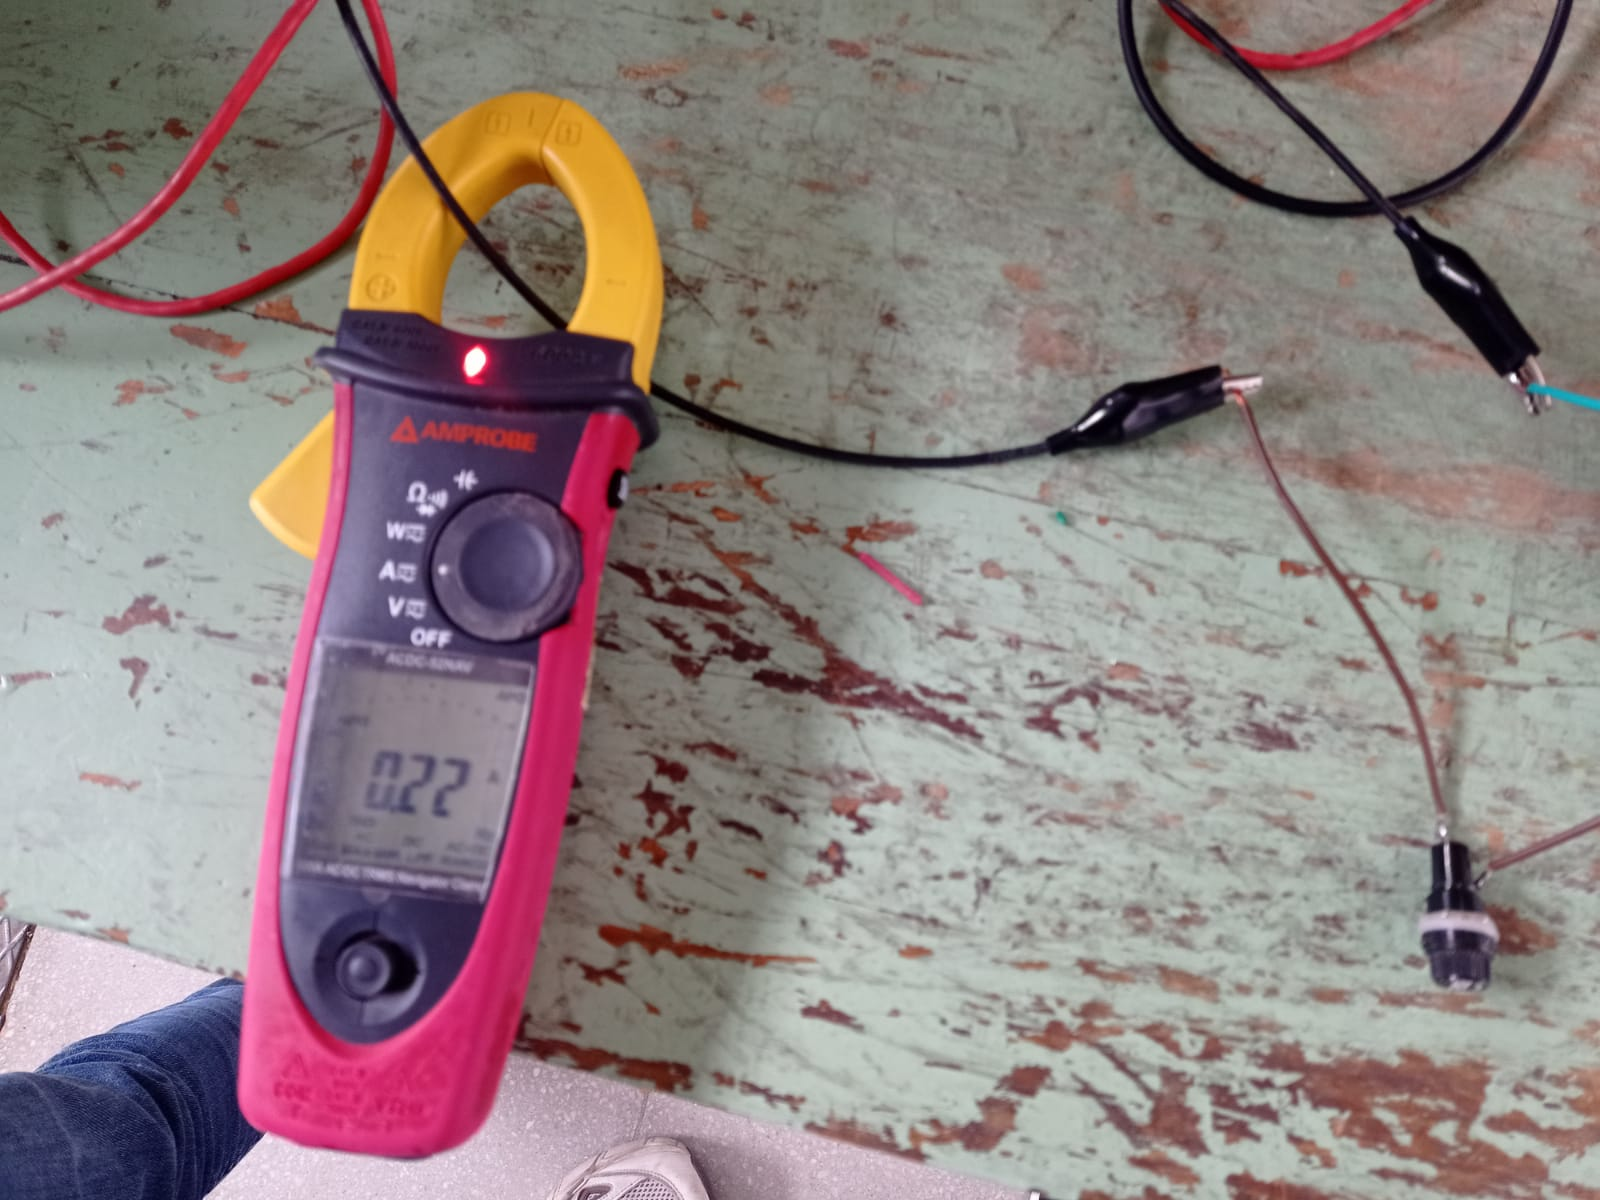
\includegraphics[width=0.48\textwidth]{fot/TP2.jpeg}
    \caption{Prueba en el laboratorio de alta tensión.}
    \label{fig:TP2}
\end{figure}


\section{analisis de resultados}
\subsection{Resultados de la prueba de circuito abierto}
Al realizar la prueba de circuito abierto, se observa que la tensión en el lado primario es de 119.9 V y la tensión en el lado secundario es de 49.91 V, lo que indica que la relación de transformación es de 2.402. Esto significa que el transformador está funcionando correctamente y que la relación de transformación es la esperada.
Con relación a la corriente de excitación en el lado primario es de 0.22 A, de la cual para valores nominales se esperaba que fuera de 0,4166 A. para lo cual se tiene que la corriente de excitación es 52.8\% lo quiere decir que la rama de magnetización tiene un valor por encima del esperado que es del 10\% respecto a la nominal%.

\subsection{Resultados de la prueba de corto circuito}
Al realizar la prueba de corto circuito, se observa que la tensión en el lado primario es de 9.24 V y la corriente en el lado del cortocircuito es de 1.03 A. Esto indica que el transformador está funcionando correctamente. Para la corriente de carga para valores nominales se tendria ques deberia ser de 1[A] por lo cual respecto a esta se tiene que la corriente de carga es del 103\% respecto a la nominal. Esto indica que el transformador está funcionando correctamente en los valores esperados.


\section{Conclusiones}
\begin{itemize}
    
    \item En cuanto a la relación de transformación, el transformador presenta valores esperados, lo que indica que el transformador está funcionando correctamente.
    \item La potencia nominal del transformador es de 50 VA, lo que indica que el transformador está diseñado para manejar esta potencia sin problemas y que no se espera que se produzcan sobrecalentamientos o fallas en el transformador si se dimensiona un uso para estos valores.
    \item El transformador presenta valores por encima de lo esperado para la corriente de la rama de magnetización esto podría deberse a los ciclos de histéresis y corrientes parásitas principalmente el primer caso, lo que provoca que la corriente de excitación sea mayor a la esperada. 
    \item La corriente de carga es del 103\% respecto a la nominal, lo que indica que el transformador está funcionando correctamente en los valores esperados.
    \item S\item En cuanto a la relación de transformación, el transformador presenta valores esperados, lo que indica que el transformador está funcionando correctamente.e logro comprender satisfactoriamente el funcionamiento del transformador, así como su diseño y construcción. lo que a futuro nos permitiria reallizar uno en funcion de las necesidades de un circuito en particular.
\end{itemize}






\section{Anexos}
\subsection{Imágenes de la construcción del transformador}
Las imagenes de la construcción del transformador son las figuras \ref{fig:TA1} a \ref{fig:TA6}.
\begin{figure}[ht!]
    \centering
    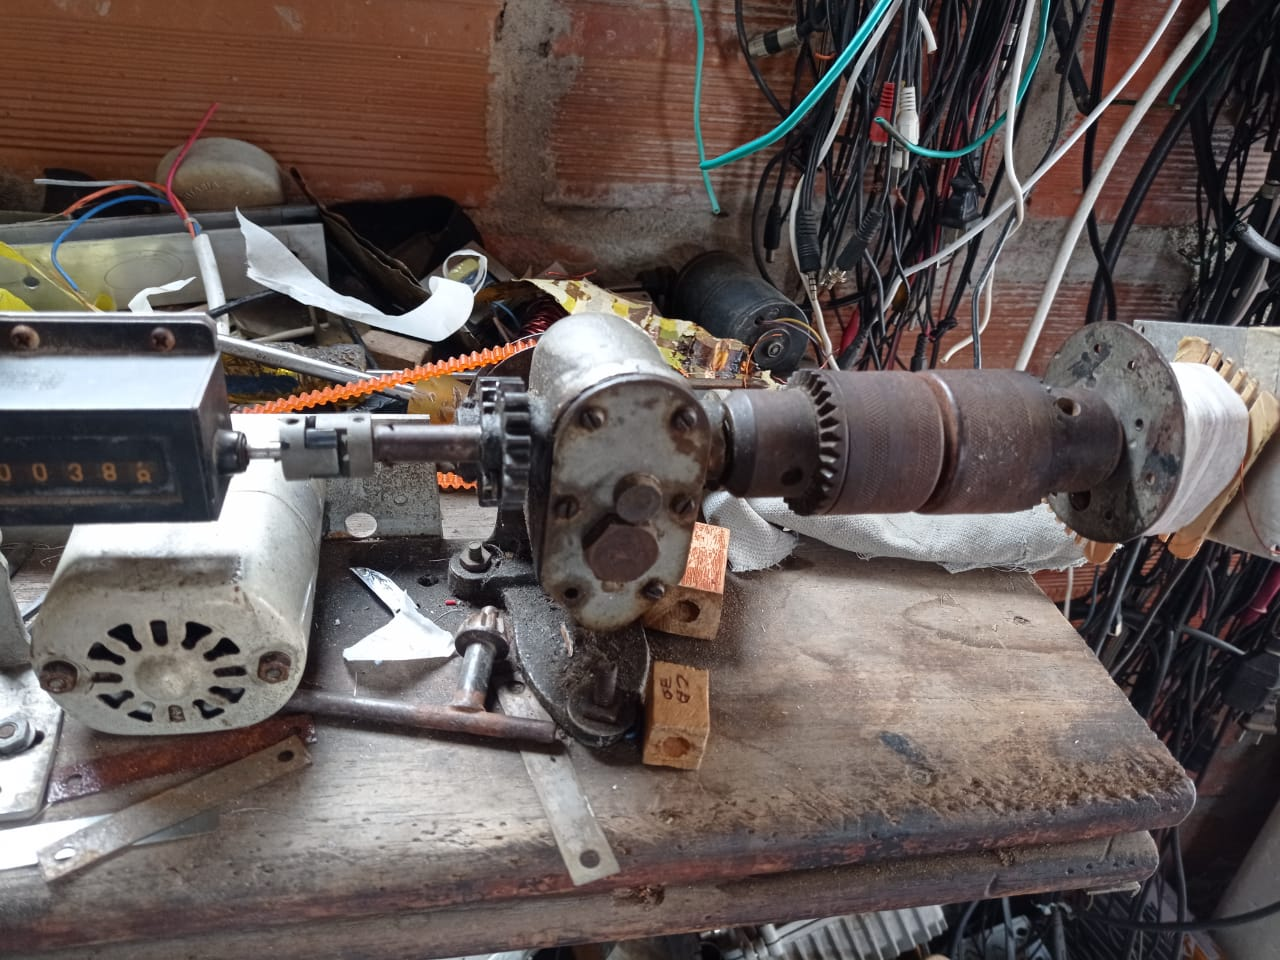
\includegraphics[width=0.48\textwidth]{fot/TA1.jpg}
    \caption{Construcción del transformador con el numero de vueltas del devanado primario mas cinta de enmascarar.}
    \label{fig:TA1}
\end{figure}

\begin{figure}[ht!]
    \centering
    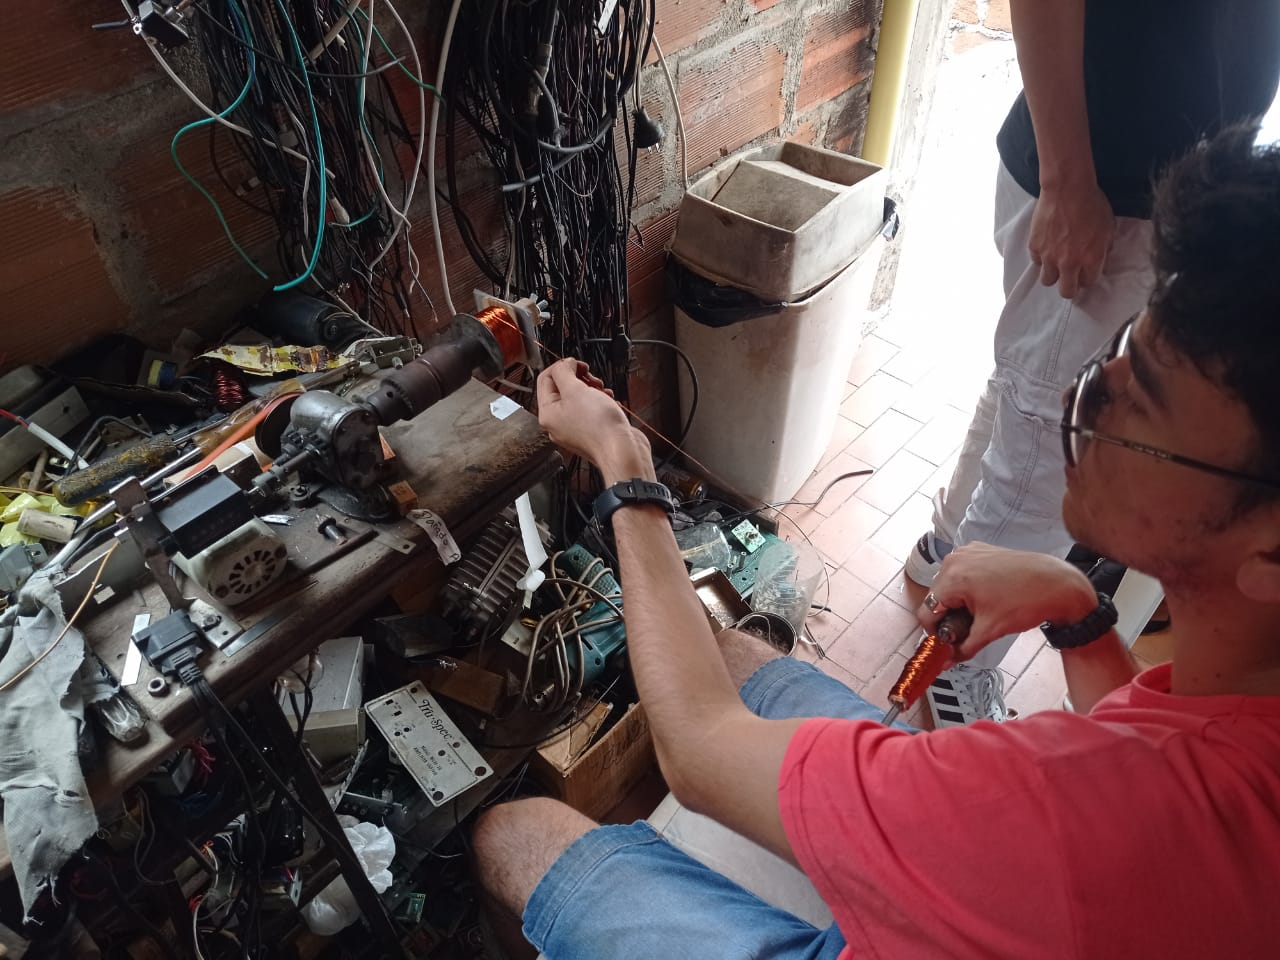
\includegraphics[width=0.48\textwidth]{fot/TA2.jpeg}
    \caption{Construcción del transformador.}
    \label{fig:TA2}
\end{figure}

\begin{figure}[ht!]
    \centering
    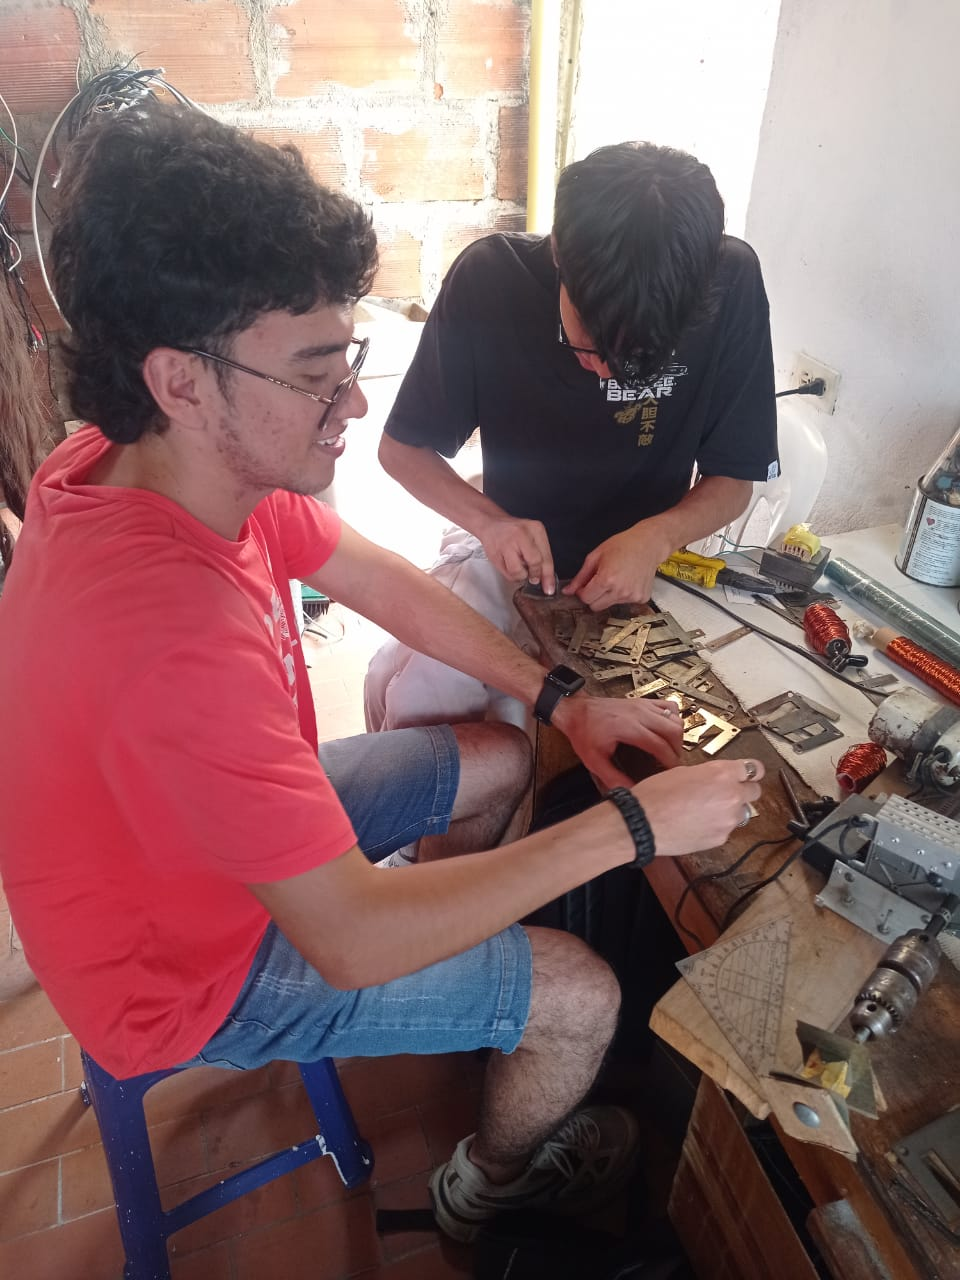
\includegraphics[width=0.48\textwidth]{fot/TA3.jpeg}
    \caption{Construcción del transformador .}
    \label{fig:TA3}
\end{figure}

\begin{figure}[ht!]
    \centering
    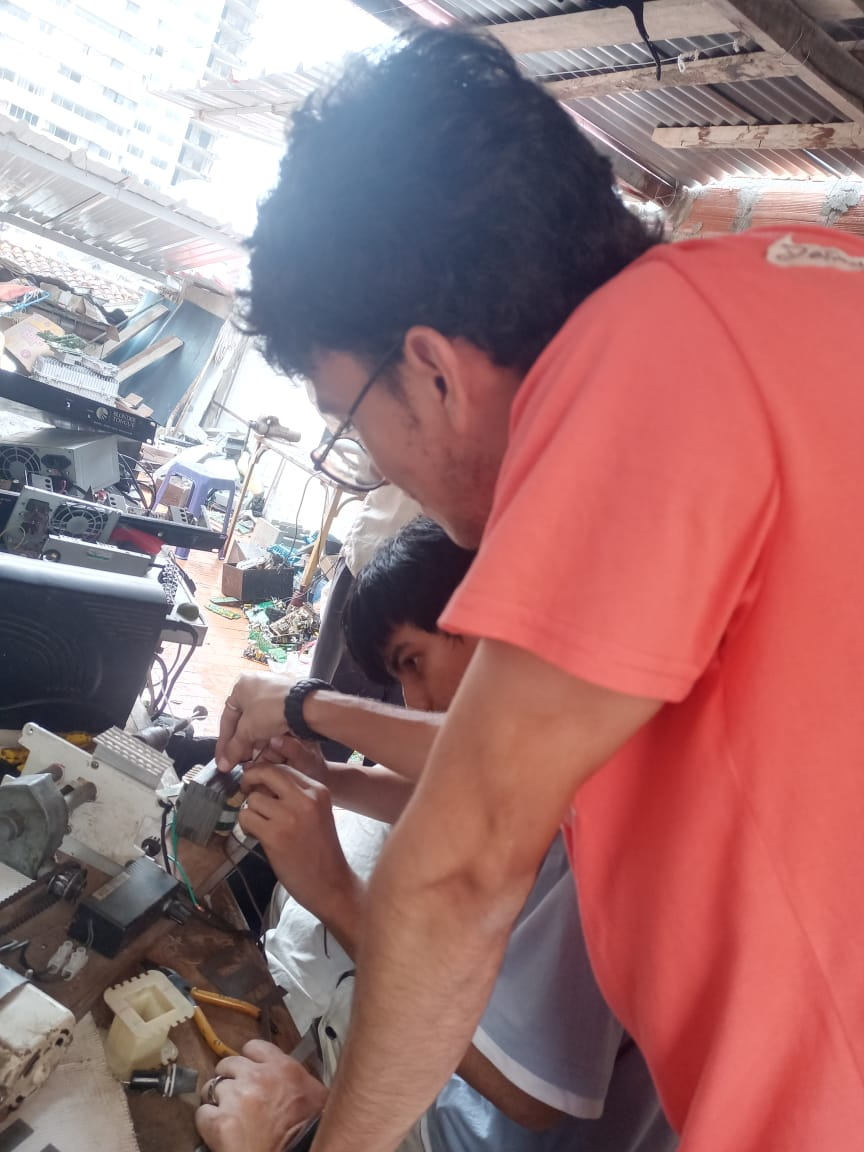
\includegraphics[width=0.48\textwidth]{fot/TA4.jpeg}
    \caption{Construcción del transformador.}
    \label{fig:TA4}
\end{figure}

\begin{figure}[ht!]
    \centering
    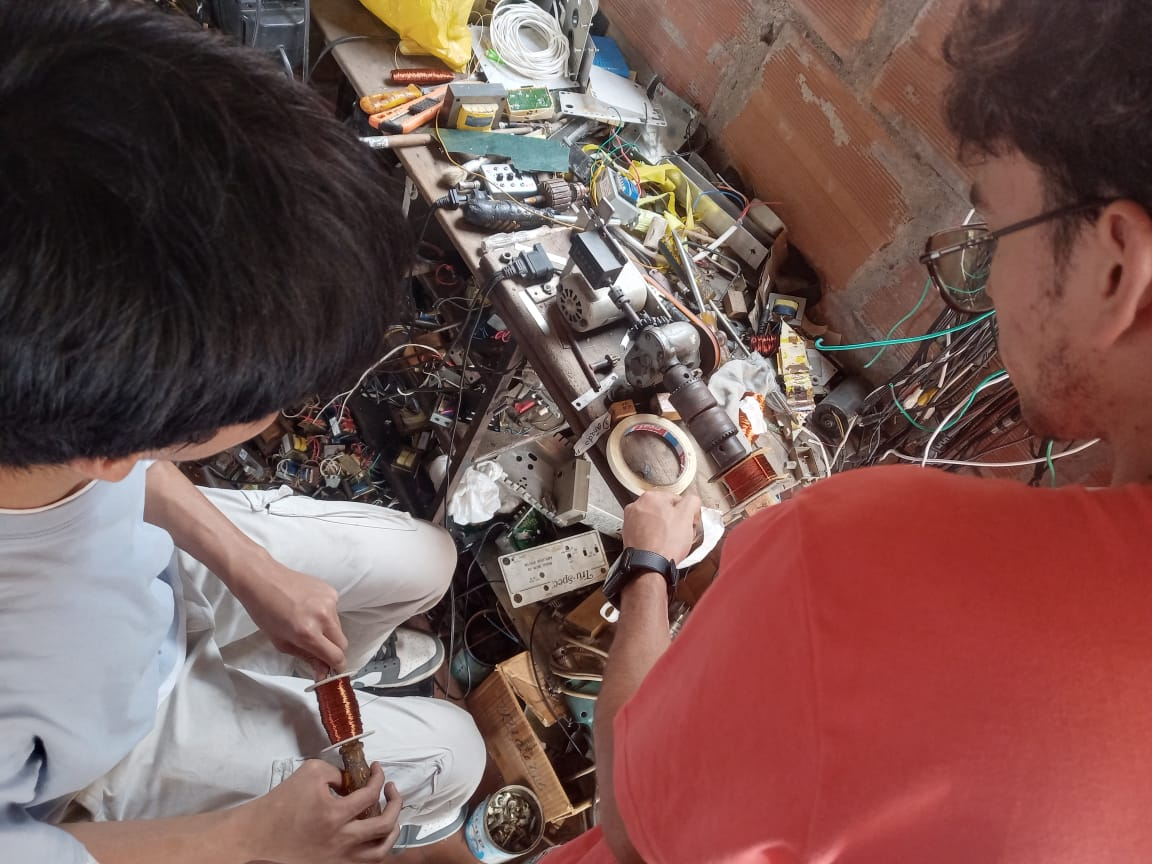
\includegraphics[width=0.48\textwidth]{fot/TA5.jpeg}
    \caption{Construcción del transformador.}
    \label{fig:TA5}
\end{figure}

\begin{figure}[ht!]
    \centering
    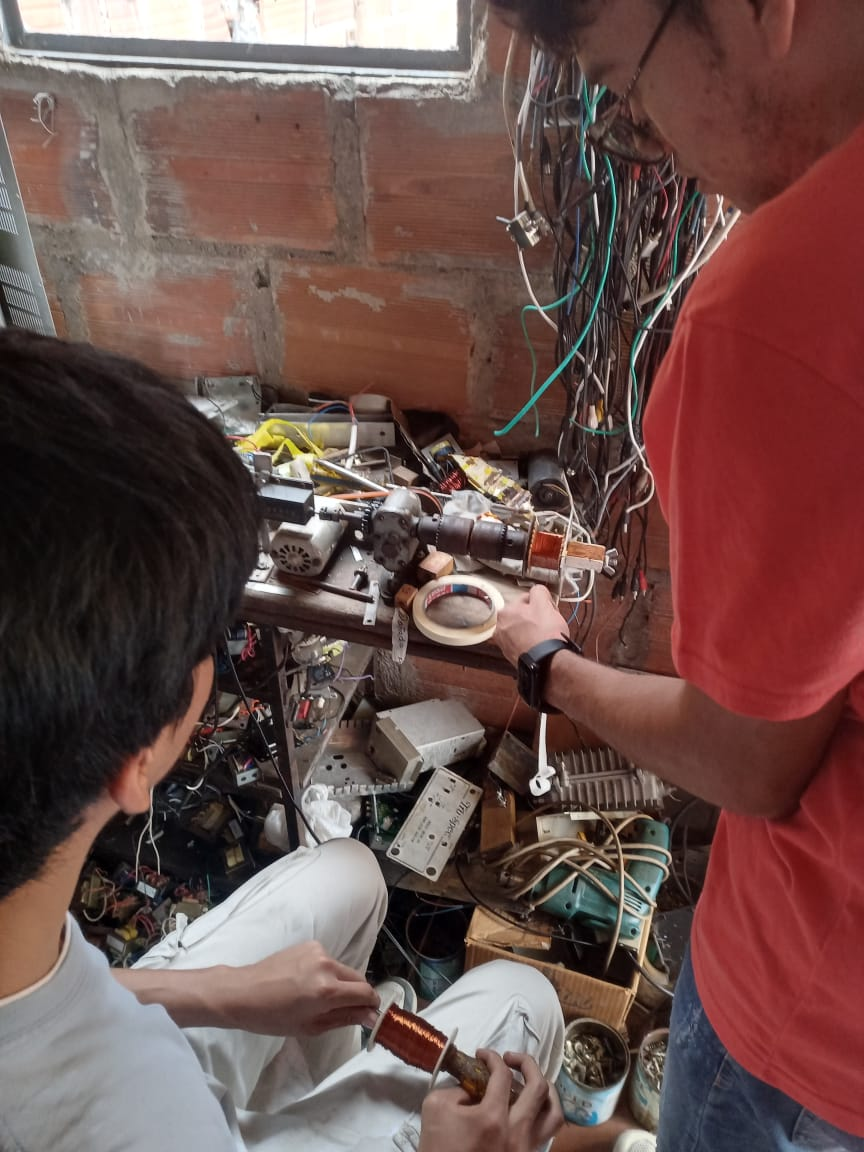
\includegraphics[width=0.48\textwidth]{fot/TA6.jpeg}
    \caption{Construcción del transformador.}
    \label{fig:TA6}
\end{figure}

         % Add the bibliography file in the preamble (correct usage)
        %\section*{Nomenclature}
        %    \addcontentsline{toc}{section}{Nomenclature}
        %    \begin{IEEEdescription}[\IEEEsetlabelwidth{$V_1,V_2,$}]
        %    \item[\smash{\begin{IEEEeqnarraybox*}[][t]{l}
        %    V_1,V_2,\\
        %    \hphantom{V_1,{}}V_3
        %    \end{IEEEeqnarraybox*}}] Three-phase PWM output line voltages.\\
        %    \mbox{}
        %    \item[$\theta$] Rotor angle (in ``electrical degrees'').
        %    \item[$\omega$] Rotor (electrical) speed, corresponding to the time
        %    derivative of $\theta$.
        %    \end{IEEEdescription}

        %    \begin{IEEEitemize}
        %        \item First item
        %        \item Second item
        %    \end{IEEEitemize}

            
        %    \begin{IEEEenumerate}
        %        \item First item
        %        \item Second item
        %    \end{IEEEenumerate}
        %    
        %    \begin{IEEEdescription}
        %        \item First item
        %        \item Second item
        %    \end{IEEEdescription}


        %   \begin{IEEEproof}
        %        The statement is true.
        %   \end{IEEEproof}


        \begin{thebibliography}{1}
            
            \bibitem{F1883}
            ASTM International, \emph{F1883 Standard Practice for Selection of Wire and Cable Size in AWG or Metric Units}, 1998. doi: 10.1520/F1883-98.
            \label{F1883}

            \bibitem{GonzalezGarcía2008}
            C. E. Gonzalez Aguas and O. García Colmenares, \emph{Guía para el diseño de núcleos de transformadores de distribución}, Trabajo de grado para optar al título de Ingeniero Electricista, Director H. R. Vargas Torres, Escuela de Ingenierías Eléctrica, Electrónica y Telecomunicaciones, Universidad Industrial de Santander, Bucaramanga, 2008.
            \label{GonzalezGarcía2008}

            \bibitem{Fraile2008}
            J. Fraile Mora, \emph{Máquinas Eléctricas}, 6ª ed. Madrid, España: McGraw-Hill, 2008.
            \label{Fraile2008}

        \end{thebibliography}

        \end{document}  
